% Section 9. Owners: growth rates each person for own algorithms; 9.1 Abhishek; 9.2-9.3 Kushagra.
\section{Performance Analysis}
\label{sec:performance}

\subsection{Growth Rate of the Major Algorithms}
\emph{Leases.} Granting a lease is $O(1)$; the leader's expiry scan grows linearly with the open units and active leases, $O(U + A)$ per one-second tick, and each expired lease costs one replicated table change, independent of the number of volunteers.

\emph{Majority voting.} Computation grows linearly with the replication factor: each unit runs between $q$ and $r$ times (2 and 3 by default, 2.0 to 2.6 measured), plus two executions for every round without a majority. The leader's voting work is $O(r)$ per result, hence $O(r^2)$ per unit, which is negligible for $r = 3$.

\emph{Resource discovery.} Each work request costs the leader $O(Ur)$ to build the candidates from $U$ open units and $O(Uf)$ for the end-of-work check with $f$ active fast volunteers, while trust updates are $O(1)$. Because every unit needs at least $q$ requests, scheduling a backlog of $U$ units costs $O(U^2 r)$ in total when all of them are open at once; we did not measure this cost separately from the other per-request work.

\emph{Leader election.} An election with $n$ coordinators costs $n-1$ messages in the best case and $O(n^2)$ in the worst case, and in steady state the leader sends $n-1$ heartbeats per interval; neither cost depends on the number of volunteers, units or jobs. \emph{Replication.} Each change costs $n-1$ messages and one round trip to the fastest backup, and the number of changes grows linearly with the number of units times the copies per unit. A catch-up snapshot is linear in the size of the task table, so this is the only part of failover whose cost grows with the workload. Once a job finishes, the table keeps only its merged result and the hashes of its unit outputs, so the table grows by about one merged result per job (Section~\ref{sec:metrics}).

\subsection{Overall Result and Reflection}
SpareCycles meets its goals on a local cluster. All six algorithms and the security layer are written by the team, each failure scenario runs and passes with one command, and all 16 test cases pass. A crashed volunteer is declared dead within 3\,s with demonstration settings, a volunteer that returns only wrong results never changes the output and is blocked after its second wrong result, and a crashed leader is replaced 2.5\,s after the crash without losing accepted work. The price is throughput: with four volunteers, majority voting delivers 68\% of the baseline.

Looking back, the \emph{pull model} kept the leader simple, since it never tracks idle volunteers, but an idle volunteer polls every second, and with a single client the volunteers sat idle between jobs. \emph{Three copies with two of three agreeing} caught every wrong result in our runs, including those that arrived as late copies, yet every unit ran 2.0--2.6 times, which is the main cost of fault tolerance. \emph{Bully with terms and a leader lease} gave a predictable leader and a fast failover, but the textbook algorithm alone would have been unsafe; terms, majority acceptance and the lease were needed to make it so, and because Bully ignores how current a node's table is, a new leader must catch up before it acts. \emph{Primary-backup replication with one backup acknowledgement} tolerates the loss of any one coordinator at the latency of a single round trip, but it holds the commit lock during that round trip; since our load tests ran with one coordinator, their numbers do not include this cost. \emph{SWIM} paid off twice: it freed the work of a crashed volunteer in seconds instead of minutes, and after a failover it freed the units leased to the volunteers' old identifiers. Finally, the \emph{stub-first workflow} let three people work in parallel behind stable interfaces on a system that ran end to end from the start, and the end-to-end scripts found problems that unit tests had missed: the first run of the faulty-volunteer scenario failed because a faulty volunteer that always ran the third copy was never compared, which led to the checking of late copies, and a leader crash under sustained load on the Docker cluster showed that the task table grew without bound (Section~\ref{sec:metrics}).

\subsection{Metrics and Comparison with a Baseline}
\label{sec:metrics}
Every coordinator exports Prometheus metrics for its main events, including accepted units, jobs, gossip members by state, lease releases, wrong results, elections, failover time and replication time, together with the standard process metrics. Fig.~\ref{fig:prometheus} shows three of them during a five-minute run on the Docker Compose cluster of three coordinators and three volunteers, with two clients submitting jobs continuously. We killed one volunteer after 90\,s and the leader, node~3, 90\,s later. The three coordinators declared the volunteer dead 7.8 to 9.0\,s after their last contact with it, with the default gossip settings, and each then counted one live member less. Node~2 became leader 2.3\,s after the crash and continued from table index 26\,273, and the clients finished 447 jobs over the whole run. Throughput under the new leader recovered slowly, because a unit needs two matching copies and the second surviving volunteer registered with the new leader only about 18\,s after the takeover.

\begin{figure*}[t]
\centering
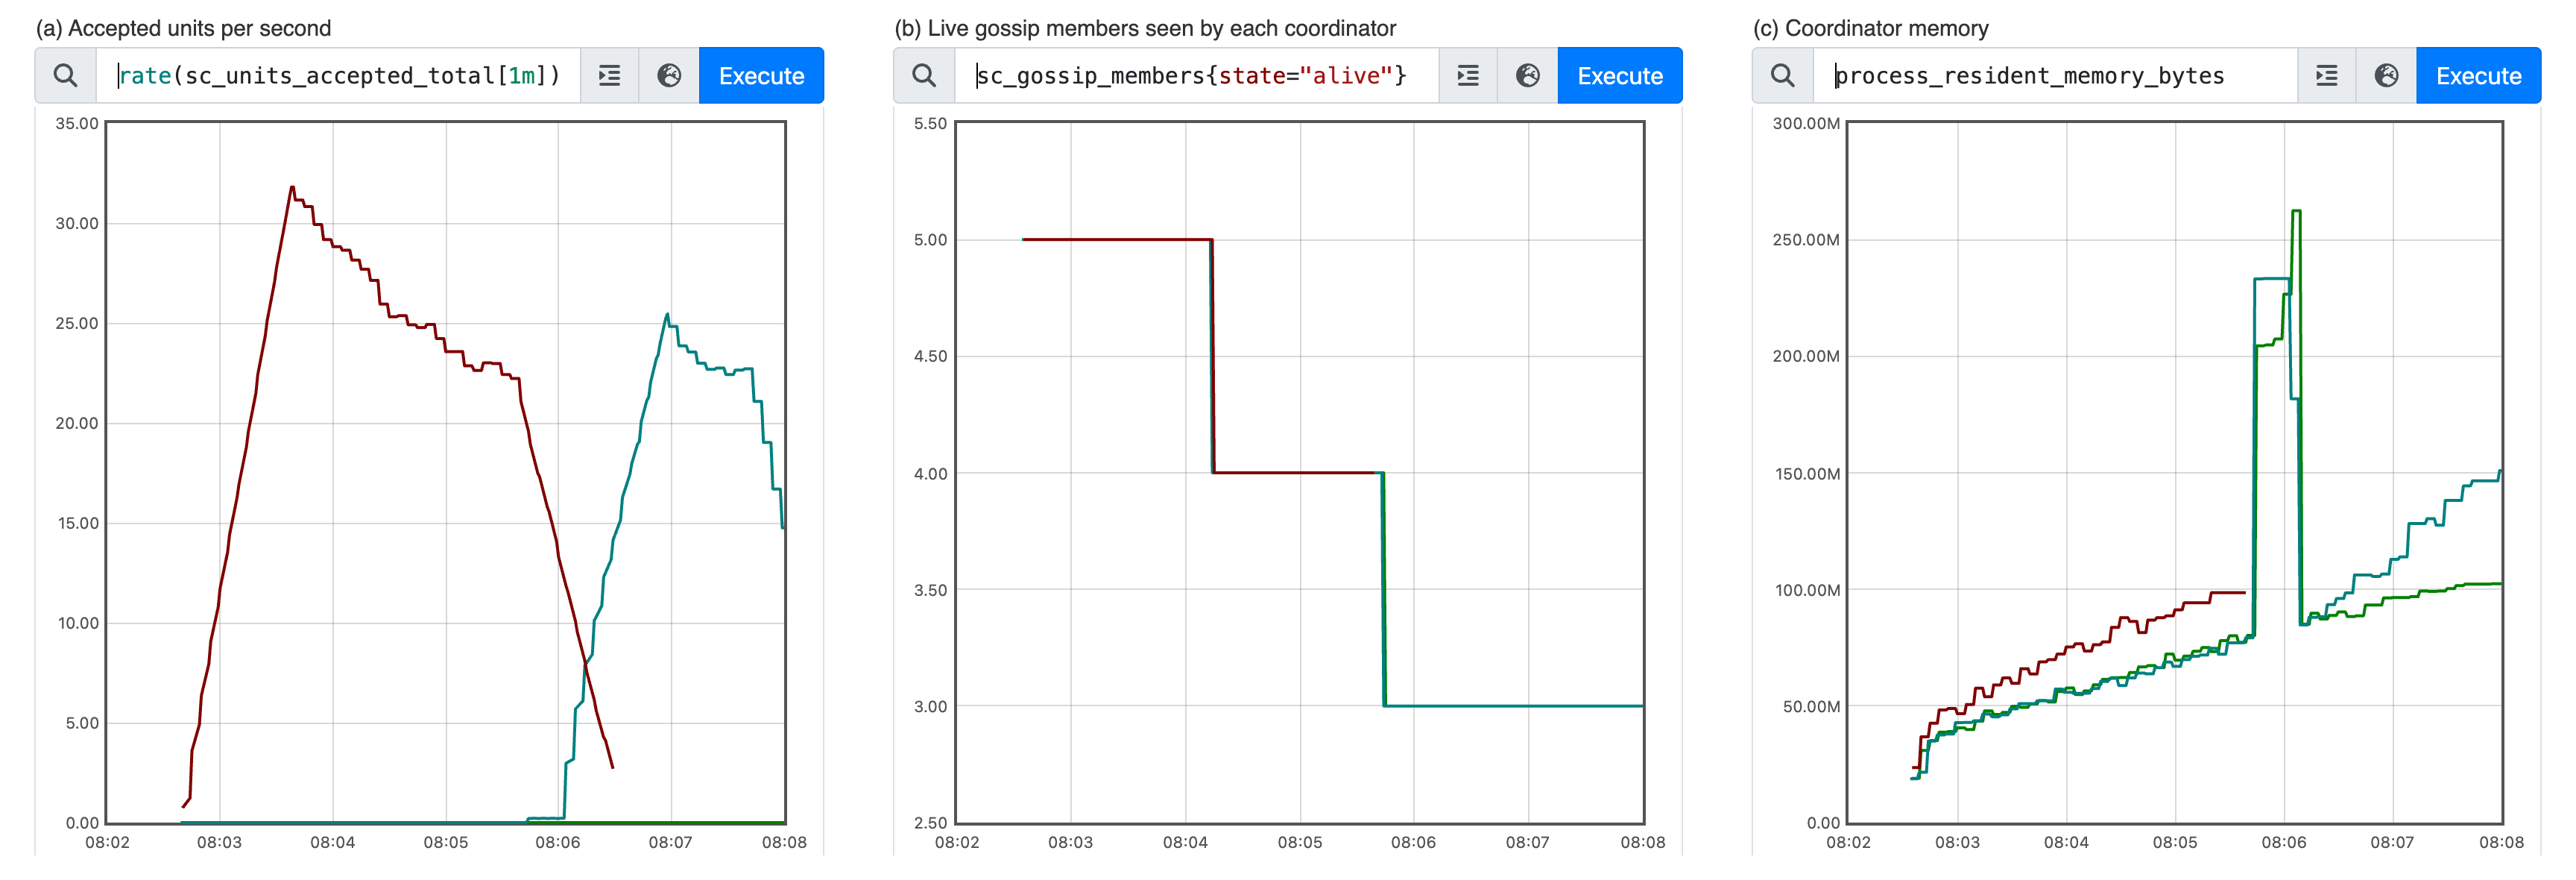
\includegraphics[width=\textwidth]{s5-prometheus.png}
\caption{Prometheus during five minutes of load on the Docker Compose cluster (times in UTC). A volunteer is killed at 08:04:08 and the leader, coordinator~3, at 08:05:38; the load stops at 08:07:38. Colors: coordinator~1 green, 2 teal, 3 red. (a) Accepted units per second, averaged over one minute, move from coordinator~3 to coordinator~2. (b) Each coordinator sees one live gossip member less after each crash. (c) Memory stays below 270\,MB, including the catch-up after the failover.}
\label{fig:prometheus}
\end{figure*}

The memory panel records a problem that this run found. In its first attempt, the task table kept every finished job with all its unit outputs and copies, 3 to 4\,MB for each fractal job, and each coordinator grew by 7 to 9\,MB/s to 1.2--1.6\,GB within three minutes. At the leader crash, Docker stopped both remaining coordinators for lack of memory. In a repeat with the crash after 80\,s, when each table held about 0.7\,GB, building, sending and loading the catch-up snapshot raised the two to 3.4 and 3.75\,GB; Docker stopped the new leader, and the last coordinator, without a majority, could not elect a leader. The local failure scenario (Section~\ref{sec:scenario-leader}) had passed because its table was small. The table now drops each unit's payload and copy outputs when the unit is accepted, and the accepted outputs when the job finishes, keeping only their hashes, which suffice to check late copies. With this change, the same run stayed at 80--100\,MB per coordinator after three minutes, and the catch-up peaked at 260\,MB. The merged result of each job, about 50\,kB for a fractal image, still stays in the table so that the client can fetch it; a long-running deployment would also need to remove finished jobs.

We measure throughput as accepted units per second and jobs per minute, and latency as the time from submitting a job to its result (mean and 95th percentile). To isolate the cost of fault tolerance, we compare two configurations of the same system on the same hardware: \emph{baseline}, in which each unit runs on one volunteer with no redundancy, and \emph{full}, in which each unit is sent to three different volunteers as majority voting requires. The baseline corresponds to a classic master--worker system without replication; the full configuration corresponds to BOINC-style redundant computing~\cite{anderson2004boinc}.

% Section 9.3 (part of 09-performance.tex). Owner: Kushagra. Data: results/load.csv, docs/test-results.md TC-07, TC-08, TC-11.
\subsection{Simulated Workloads}
A load generator submits eight fractal jobs of 64 units each (a $1024\times1024$ image in $128\times128$ tiles, 2000 iterations) against one coordinator. All processes run on one laptop with 10 cores (Apple silicon), started in the foreground from a terminal. At the time of measurement, the full configuration accepted the first returned result instead of waiting for a two-of-three majority; it therefore measures the cost of running three copies, which dominates the cost of voting. A repeated run differed by less than 0.2\%.

\paragraph{More volunteers}
With two clients submitting at the same time, we vary the number of volunteers (Table~\ref{tab:load}, Fig.~\ref{fig:load}). The baseline grows from 69 to 110 and 140 units per second, a factor of 2.0 for four volunteers. The shortfall from a factor of four has a clear cause: in this test a unit computes for only about 15\,ms, whereas the design targets units of about 60\,s, so the per-unit messages to the coordinator (a request, a result and two replicated table changes) are a large share of the cost. With realistic units this overhead would be negligible.

The full configuration behaves as a simple model predicts. With $N$ volunteers and three copies per unit, each unit occupies $\min(N,3)$ volunteers, so the useful throughput is about $N/\min(N,3)$ times that of a single volunteer. For $N=1$ and $N=2$ this means no gain over one volunteer, and indeed the full configuration delivers 68.2 and 69.2 units per second, the same as one baseline volunteer. With four volunteers it reaches 74.1 units per second, 53\% of the baseline, so fault tolerance costs 47\% of the throughput. For $N \ge 3$ the model predicts a share of one third, because every unit costs three executions however large the pool is; the measured share is higher because the baseline itself scales sublinearly in this test. This is the price of tolerating a malicious volunteer with replication. Two refinements could reduce it: adaptive replication, which BOINC applies to hosts with a good history, and early cancellation of the remaining copies once a majority agrees.

\begin{table}[t]
\centering
\caption{Throughput and job time with more volunteers (8 jobs, 512 units, 2 clients)}
\label{tab:load}
\begin{tabular}{@{}lrrrrr@{}}
\toprule
Mode & Vol. & Units/s & Jobs/min & Mean (s) & p95 (s) \\
\midrule
baseline & 1 & 69.1 & 64.8 & 1.75 & 2.55 \\
baseline & 2 & 109.6 & 102.8 & 1.12 & 2.14 \\
baseline & 4 & 139.6 & 130.8 & 0.89 & 1.64 \\
full & 1 & 68.2 & 63.9 & 1.76 & 2.45 \\
full & 2 & 69.2 & 64.9 & 1.75 & 2.55 \\
full & 4 & 74.1 & 69.5 & 1.63 & 2.15 \\
\bottomrule
\end{tabular}
\end{table}

\begin{figure}[t]
\centering
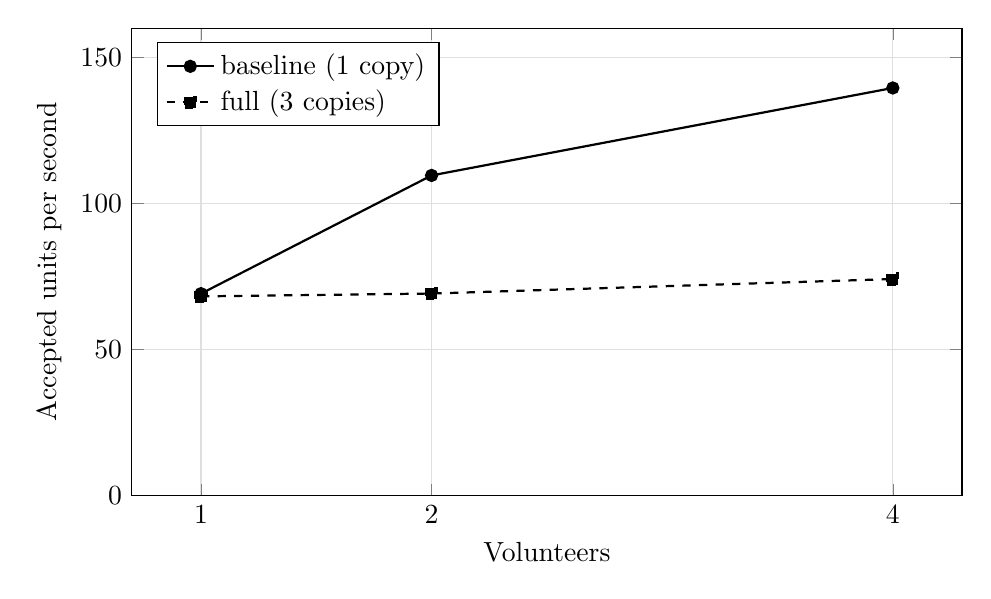
\begin{tikzpicture}
\begin{axis}[
  width=\columnwidth, height=0.62\columnwidth,
  xlabel={Volunteers}, ylabel={Accepted units per second},
  xtick={1,2,4}, ymin=0, ymax=160,
  legend pos=north west, legend cell align=left,
  grid=major, grid style={gray!25}]
\addplot[mark=*, thick] coordinates {(1,69.137) (2,109.607) (4,139.550)};
\addlegendentry{baseline (1 copy)}
\addplot[mark=square*, thick, dashed] coordinates {(1,68.207) (2,69.176) (4,74.142)};
\addlegendentry{full (3 copies)}
\end{axis}
\end{tikzpicture}
\caption{Throughput as volunteers are added, with 2 clients. Data: \texttt{results/load.csv}.}
\label{fig:load}
\end{figure}

\paragraph{More users}
With four volunteers in the full configuration, we vary the number of clients that submit jobs at the same time (Table~\ref{tab:clients}, Fig.~\ref{fig:clients}). With one client, the volunteers sit idle while a job is submitted, split and polled, so throughput is only 42.5 units per second. Two clients keep the volunteers busy, and throughput rises to 73.1. Beyond that it stays flat: the volunteers are the bottleneck, at about 75 units per second. Job time then grows with the number of clients, from a mean of 1.5\,s with one client to 4.7\,s with eight, as more jobs share the same volunteers; this is the expected queueing behavior. With eight clients, throughput falls slightly to 68.1 units per second, as more jobs and more polling compete for the single coordinator.

\begin{table}[t]
\centering
\caption{Throughput and job time with more clients (4 volunteers, full mode, 8 jobs)}
\label{tab:clients}
\begin{tabular}{@{}rrrrr@{}}
\toprule
Clients & Units/s & Jobs/min & Mean (s) & p95 (s) \\
\midrule
1 & 42.5 & 39.8 & 1.51 & 2.03 \\
2 & 73.1 & 68.5 & 1.64 & 2.25 \\
4 & 77.4 & 72.6 & 2.75 & 3.57 \\
8 & 68.1 & 63.9 & 4.66 & 7.52 \\
\bottomrule
\end{tabular}
\end{table}

\begin{figure}[t]
\centering
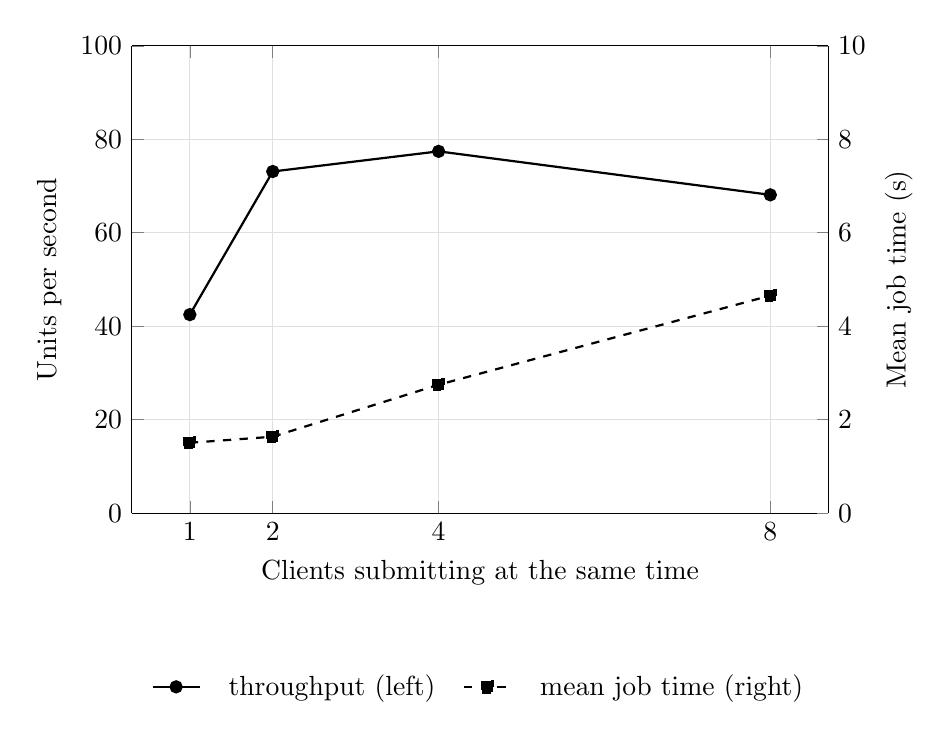
\begin{tikzpicture}
\begin{axis}[
  width=0.86\columnwidth, height=0.62\columnwidth,
  xlabel={Clients submitting at the same time}, ylabel={Units per second},
  xtick={1,2,4,8}, ymin=0, ymax=100,
  axis y line*=left,
  grid=major, grid style={gray!25}]
\addplot[mark=*, thick] coordinates {(1,42.489) (2,73.111) (4,77.420) (8,68.116)};
\end{axis}
\begin{axis}[
  width=0.86\columnwidth, height=0.62\columnwidth,
  xtick={1,2,4,8}, xticklabels={}, ymin=0, ymax=10,
  axis y line*=right, axis x line=none,
  ylabel={Mean job time (s)},
  legend style={at={(0.5,-0.32)}, anchor=north, legend columns=2, draw=none, column sep=8pt}]
\addlegendimage{mark=*, thick}
\addlegendentry{throughput (left)}
\addplot[mark=square*, thick, dashed] coordinates {(1,1.506) (2,1.637) (4,2.749) (8,4.656)};
\addlegendentry{mean job time (right)}
\end{axis}
\end{tikzpicture}
\caption{Throughput and job time as more users submit jobs (4 volunteers, full mode). Data: \texttt{results/load.csv}.}
\label{fig:clients}
\end{figure}

